\chapter{Correspondencia de parámetros entre los modelos microscópico y macroscópico}
\label{cap:redNeuronal}

En los Capítulos \ref{cap:descripcionTrabajo} y \ref{cap:modeloMacroscopico} se establece el marco teórico de dos modelos matemáticos que dan una posible explicación del mecanismo que rige la dinámica de población de las células T durante una infección aguda. Como se puede ver en las simulaciones correspondientes de estos modelos (ver Capítulo \ref{cap:simulaciones} y Sección \ref{sec:simu_macro}) ambos pueden reproducir comportamientos similares, como son el de tolerancia e intolerancia al \textit{patógeno}. Sin embargo, ambos modelos son notablemente distintos por dos razones principalmente: 

\begin{enumerate}
	\item El punto de vista desde el cual se aborda el algoritmo de decisión de las células T es distinto. Mientras que el modelo microscópico determina el algoritmo de comportamiento de cada célula de manera individual, el macroscópico presenta unas ecuaciones que gobiernan sobre toda la población de células. 
	
	\item Las ecuaciones diferenciales que conforman el modelo microscópico son de primer orden y su significado, desde el punto de vista biológico está bien definido. Esto es, los parámetros de este modelo, tales como el número de receptores de membrana de la célula ($r_{i}$) o la tasa de cambio de estos receptores ($\lambda_{xy}$) (ver Tabla \ref{tabla:param}), constituyen conceptos biológicos claros. Por su parte, el modelo macroscópico utiliza un sistema de ecuaciones de segundo grado, basado en las dinámicas \textit{newtonianas} y en dos propiedades de la población: la elasticidad y la inercia. Los parámetros $k$ y $\lambda$ representan estas dos últimas propiedades en las ecuaciones, respectivamente. Sin embargo, desde el punto de vista biológico, el valor de estos parámetros tiene un significado difuso, pues no se conocen mecanismos que rijan estas dos propiedades.
	
	%pues cada célula contiene muy poca información sobre el avance de la infección y es improbable que cada célula pueda medir  
\end{enumerate}

A pesar de que el número de parámetros del modelo macroscópico es considerablemente menor, la elección de los parámetros $k$ y $\lambda$ es más compleja que la de los parámetros del modelo microscópico por la razón $2$. Así las cosas, lo ideal sería poder establecer una correspondencia entre los parámetros de ambos modelos. De esta manera se podrían establecer los valores de los parámetros del modelo microscópico, que tienen un significado biológico claro, e inferir el valor de los parámetros del modelo macroscópico o viceversa. A lo largo de este capítulo se detalla cómo se a abordado este problema mediante el uso de técnicas de inteligencia artificial (Sección \ref{sec:conjDatos_entreRed}) y se interpretan los resultados obtenidos (Sección \ref{sec:resultadoRed}). 


\section{Conjunto de datos y entrenamiento de la red neuronal}
\label{sec:conjDatos_entreRed}
%Como ya se avanzaba en la introducción, este problema se ha atajado mediante el uso de inteligencia artificial, más concretamente de una red neuronal.

Como una primera aproximación a esta cuestión de correspondencia de parámetros, se propone la implementación de una red neuronal cuyo propósito es predecir el valor de los parámetros que se le deben asignar al modelo macroscópico teniendo como entrada aspectos característicos de una simulación. En otros términos, se podría decir que se busca hacer la función inversa del modelo. De esta manera, podemos hacer una simulación con unos parámetros concretos del modelo microscópico y obtener el valor de los parámetros del modelo macroscópico que se deberían usar para lograr un resultado similar. 

Antes de poder implementar la red es necesario determinar con qué datos se va a trabajar. Más concretamente se deben establecer las entradas y las salidas que tendrá la red. En nuestro caso se toman las siguientes decisiones:


\begin{itemize}
	\item Las simulaciones que se realizan para obtener los datos pertinentes se corresponden con situaciones de intolerancia al \textit{patógeno}.
	
	\item La red neuronal consta de diez datos de entrada y cuatro de salida. Los seis primeros datos de entrada se corresponden con seis puntos de interés de cada simulación. Estos puntos son: el máximo número de células de patógeno alcanzado, el máximo número de células T alcanzado, el tiempo en el que se alcanzaron ambos y el tiempo en el que desaparecieron ambas poblaciones (en la Figura \ref{fig:red_micro} pueden verse destacados los puntos mencionados), que denominaremos como \textit{max\_P}, \textit{max\_T}, \textit{t\_max\_P}, \textit{t\_max\_T}, \textit{t\_min\_P}, \textit{t\_min\_T}, respectivamente. Los cuatro restantes datos de entrada son los parámetros $\alpha$, $\beta$, $k$ y $\lambda$ del modelo macroscópico con los cuales se han obtenido los seis valores anteriores. Por último, los cuatro parámetros de salida de la red se corresponden con los valores de los parámetros $\alpha$, $\beta$, $k$ y $\lambda$ predichos por la misma.
	
	\item El rango de valores para $\alpha$, $\beta$, $k$ y $\lambda$ se estableció con ayuda del modelo macroscópico adimensional (ver Figura \ref{fig:macro_toler_intoler}), para ajustarnos lo más posible a una situación de intolerancia, y de tal manera que el número de simulaciones resultantes no fuera demasiado elevado pero permitiendo suficiente variabilidad en los datos para abarcar el mayor número posible de situaciones. En concreto se establecieron los siguientes rangos:
	
	\begin{itemize}
		\item $\alpha \in  [0,75;7]$
		\item $\beta \in [0,1;5]$
		\item $k, \lambda \in [0,1;2]$
	\end{itemize}
	
	Con estos rangos y a un paso\footnote{Con paso nos referimos al valor del incremento del parámetro en cada iteración.} de $0,5$ se obtienen unas $2080$ simulaciones aproximadamente, de las cuales $1587$ fueron casos de intolerancia. Los valores correspondientes a los puntos de interés de la simulación y sus parámetros se recogen en el archivo \textit{data\_neural\_network\_csv} por filas y en el mismo orden que han sido mencionados (\textit{max\_P}, \textit{max\_T}, \textit{t\_max\_P}, \textit{t\_max\_T}, \textit{t\_min\_P}, \textit{t\_min\_T}, $\alpha$, $\beta$, $k$ y $\lambda$). Este documento da lugar al conjunto de datos de la red.
	
	Como es habitual para el entrenamiento de una red neuronal, el $70\%$ del conjunto de los datos, tomado de forma aleatoria, se utilizó para el entrenamiento y el $30\%$ restante para \textit{testear} la red. La implementación de la red está realizada en Python y el código correspondiente puede verse en el archivo \textit{redNeuronal\_modeloMacro.py}. Esta cuenta con cinco capas densas y activaciones \textit{ReLu}\footnote{$ReLu(x) = max(0,x)$}. Esto es importante en la última capa, puesto que los parámetros no pueden tomar valores negativos.
	
\end{itemize}


\begin{figure}[t]
	\centering
	\begin{tabular}{cc}
		\subfloat[Valores de \textit{loss} calculados para la red neuronal durante el entrenamiento.]{
			\label{fig:loss}
			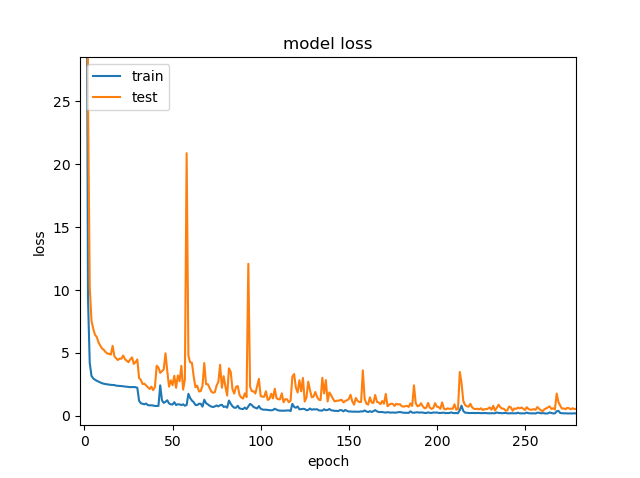
\includegraphics[width=0.5\columnwidth]{Imagenes/RedNeuronal/loss}}
		& \subfloat[Valores de \textit{accuracy} calculados para la red neuronal durante el entrenamiento.]{
			\label{fig:accuracy}
			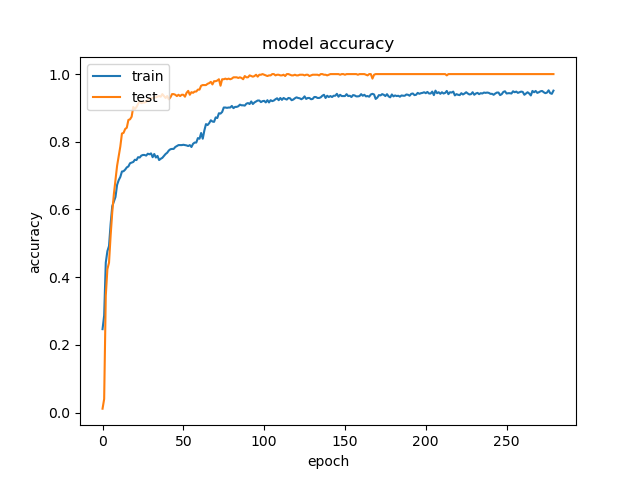
\includegraphics[width=0.5\columnwidth]{Imagenes/RedNeuronal/accuracy}}\\
	\end{tabular}
	\caption{Representación gráfica de los valores de \textit{loss} y \textit{accuracy} para cada \textit{epoch} durante el entrenamiento de la red.}
	\label{fig:loss_accuracy}
\end{figure}


\section{Resultados obtenidos por la red neuronal}
\label{sec:resultadoRed}

En esta sección se exponen los resultados obtenidos tras el entrenamiento de la red, prestando atención a los valores de \textit{loss} y \textit{accuracy} alcanzados. Además, veremos un ejemplo real de la inferencia de parámetros dada por la red tras establecer como entrada una simulación del modelo microscópico. 

Comencemos definiendo los conceptos de \textit{epoch}, \textit{loss} y \textit{accuracy} para una red neuronal, de esta manera las gráficas y resultados que vienen a continuación no presentarán ningún impedimento terminológico: Se entiende por \textit{epoch} cada pasada completa por todo el conjunto de datos de entrenamiento. Las redes neuronales, cuando entrenan, hacen varias pasadas por los datos y, en cada una de ellas, intentan minimizar una función de error. El concepto de \textit{loss} está asociado a esto último, pues este es el valor que intentamos minimizar. Cuanto más pequeño es más precisas son las predicciones de la red. En nuestro caso, el valor de \textit{loss} se corresponde con el error cuadrático medio. Por su parte, el valor de \textit{accuracy} es una métrica utilizada para medir el rendimiento del algoritmo. Este valor se calcula una vez la red se ha entrenado y ha fijado todos sus parámetros. El valor de \textit{accuracy} mide cómo de preciso es el modelo comparado con los datos reales. Por ejemplo, supongamos que tenemos $1000$ muestras y nuestro modelo es capaz de clasificar bien $990$ de ellas entonces, el valor de \textit{accuracy} es del $99\%$.

En la Figura \ref{fig:loss_accuracy} podemos ver las gráficas correspondientes a los valores de \textit{loss} y \textit{accuracy} durante el entrenamiento de la red. Como se puede observar en la Figura \ref{fig:loss}, el valor de \textit{loss} consigue estabilizarse al mínimo en el conjunto de prueba una vez pasada la iteración $230$ (ver Figura \ref{fig:loss}). Por su parte, el valor de \textit{accuracy} (ver Figura \ref{fig:accuracy}) continúa incrementándose para el conjunto de entrenamiento hasta prácticamente la última iteración, lo que indica que el modelo no está sobreentrenando, a pesar de que en el conjunto de prueba se estabilice una vez pasada la iteración $100$ aproximadamente. Estos resultados sugieren que el número de \textit{epoch} utilizados para entrenar la red es el óptimo.


%\begin{figure}[t]
%	\centering
%	
%	\subfloat[Valores de \textit{loss} calculados para la red neuronal durante el entrenamiento.]{
%		\label{fig:loss}
%		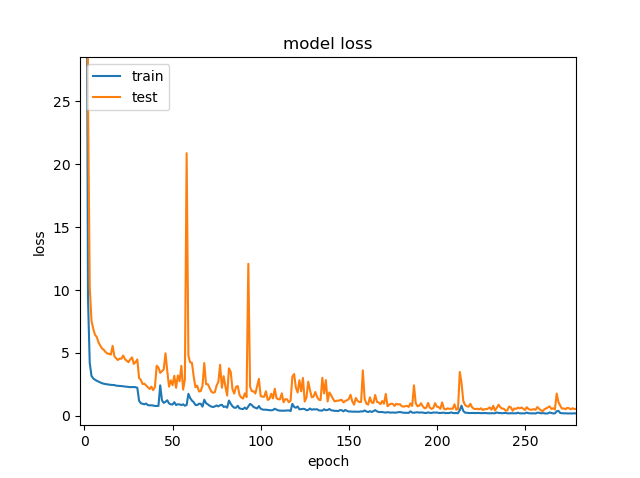
\includegraphics[width=0.6\columnwidth]{Imagenes/RedNeuronal/loss}}
%	
%	\subfloat[Valores de \textit{accuracy} calculados para la red neuronal durante el entrenamiento.]{
%		\label{fig:accuracy}
%		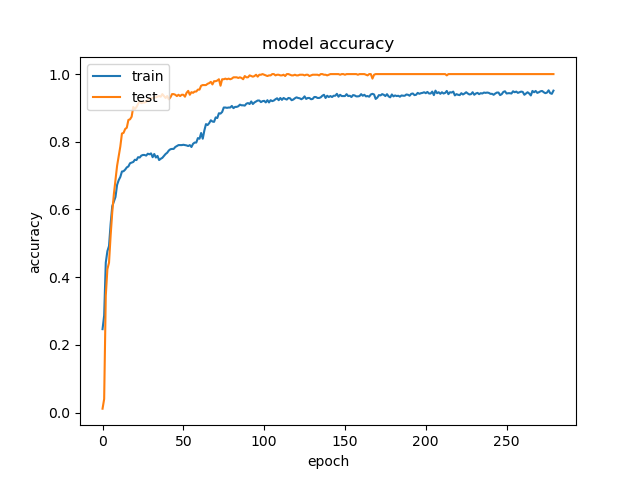
\includegraphics[width=0.6\columnwidth]{Imagenes/RedNeuronal/accuracy}}
%	
%	\caption{Representación gráfica de los valores de \textit{loss} y \textit{accuracy} para cada \textit{epoch} durante el entrenamiento de la red.}
%	\label{fig:loss_accuracy}
%\end{figure}

%AQUÍ IBA LA FIGURA DE LOSS Y ACCURACY


En el archivo \textit{resultados.txt} se pueden ver algunos de los resultados obtenidos por la red, correspondientes a distintos valores de \textit{accuracy}\footnote{El resultado de cada de las distintas simulaciones se representa por filas con el siguiente formato: [los seis puntos de interés generados tras una simulación del modelo macroscópico] $=>$ [el valor predicho por la red para los parámetros $\alpha$, $\beta$, $k$ y $\lambda$] (expected [el valor real de dichos parámetros]).}. En el caso que nos ocupa ahora, detallaremos un ejemplo concreto obtenido a partir de los datos de una simulación del modelo microscópico, cumpliendo así con el propósito de esta red. En la Figura \ref{fig:red_micro} podemos ver el resultado de la simulación del modelo microscópico, con los seis puntos de interés destacados. Concretamente el valor de esos parámetros es: $\textit{max\_P} = 74,4$, $\textit{max\_T} = 88$, $\textit{t\_max\_P} = 3,15$, $\textit{t\_max\_T} = 4,8$, $\textit{t\_min\_P} = 3,9$ y  $\textit{t\_min\_T} = 6,3$. Una vez la red estaba entrenada se introdujeron estos valores como entrada para obtener la predicción de los valores de los parámetros del modelo macroscópico. El resultado obtenido fue: $\alpha = 3,5$, $\beta = 0,29$, $k = 0,3$ y $\lambda = 0,9$. En la Figura \ref{fig:red_macro} puede verse la simulación del modelo macroscópico correspondiente a esos parámetros. Si comparamos ambas figuras observamos a simple vista que ambas presentan dos situaciones muy similares, si bien es cierto que los valores difieren ligeramente. En particular, la simulación del modelo macroscópico tiene en puntos de interés los siguientes valores: $\textit{max\_P} = 68.94$, $\textit{max\_T} = 98,82$, $\textit{t\_max\_P} = 1,27$, $\textit{t\_max\_T} =4$, $\textit{t\_min\_P} = 2,45$ y  $\textit{t\_min\_T} = 6,87$. Si comparamos estos valores con los obtenidos con el modelo microscópico vemos el valor \textit{max\_P} es menor en el modelo microscópico pero que los tiempos asociados a este (\textit{t\_max\_P} y \textit{t\_min\_P}) también lo son. Lo que nos dice que, a pesar de que los valores no han sido exactos, la forma de la gráfica sí se preserva. Si prestamos atención a los valores referentes a las células T, vemos que el patrón ha cambiado, pues se alcanza un número mayor de células T en el modelo macroscópico y, sin embargo, este valor se alcanza antes que en el modelo microscópico. Esto nos indica que que los parámetros de elasticidad e inercia no se han ajustado completamente, lo que hace que observemos ese pequeño desfase.



%\begin{figure}[t]
\begin{figure}[t]
	\centering
	\begin{tabular}{cc}
		\subfloat[Simulación: caso de intolerancia al \textit{patógeno} en el modelo microscópico. Parámetros y variables: $t\_cycle = 0,05$, $t\_apo = 0,1$, $t\_next = 0,15$, $\alpha = 6,4$, $\beta = 0.22$, $\lambda_{pd} = 0.05$, $\lambda_{Tp} = 6*10^{-5}$, $\lambda_{pp} = 0,5*10^{-4}$, $\mu_{pc} = 8$, $\mu_{da} = 15$.]{
			\label{fig:red_micro}
			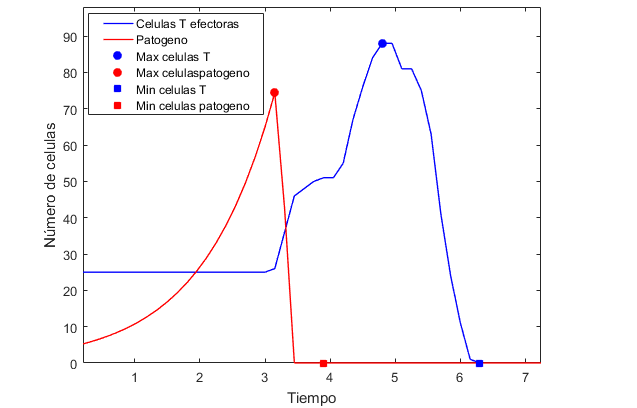
\includegraphics[width=0.5\textwidth]{Imagenes/RedNeuronal/micro}}
		& \subfloat[Simulación: caso de intolerancia al \textit{patógeno} en el modelo macroscópico. Parámetros: $\alpha = 3,5$, $\beta = 0,29$, $k = 0,3$, $\lambda = 0,9$, $P_m = 0$.]{
			\label{fig:red_macro}
			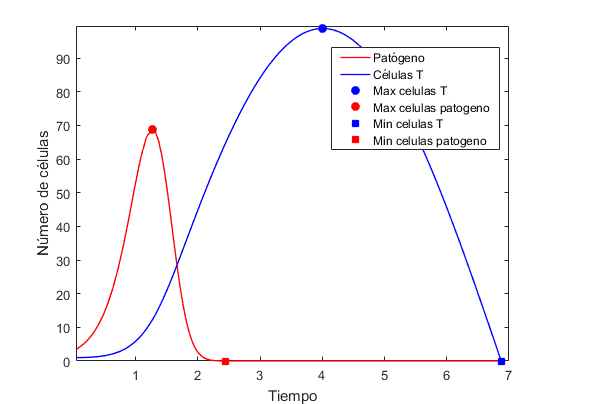
\includegraphics[width=0.5\textwidth]{Imagenes/RedNeuronal/macro}}\\
	\end{tabular}
	\caption{Ejemplo con simulaciones del modelo microscópico y macroscópico con los valores de los parámetros predichos por la red neuronal. Casos de intolerancia al \textit{patógeno}}%\label{foo}
\end{figure}



%\begin{figure}[t]
%	\centering
%	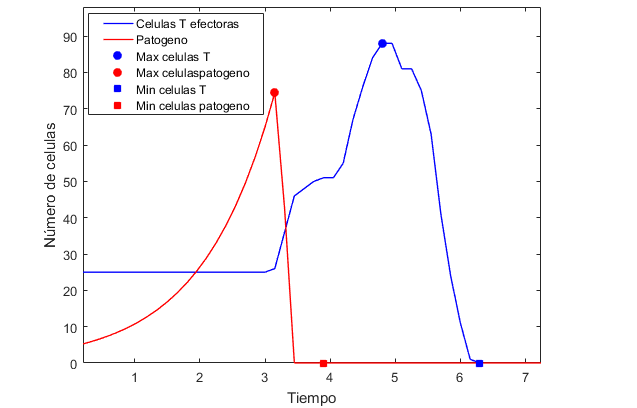
\includegraphics[width=0.7\textwidth]{Imagenes/RedNeuronal/micro}
%	\caption{Simulación: distintas poblaciones de células T con distintas afinidades al \textit{patógeno}. Clon subdominante. Los parámetros son los mismos que se exponen en la Tabla \ref{tabla:param}, excepto: $\lambda_{Tp}^{clon_2} = 10^{-5}$.}
%	\label{fig:red_micro}
%\end{figure}












